\documentclass{beamer}

\usepackage{graphicx}
\usepackage{hyperref}
\usepackage[latin1]{inputenc}
\usepackage[T1]{fontenc}
\usepackage[english]{babel}
\usepackage{listings}
\usepackage{xcolor,mathrsfs,url}
\usepackage{amssymb}
\usepackage{amsmath}
\usepackage{ifthen}

% The command to define a subsection is '\subsec{}' and NOT '\subsection'.
% This code generates the bar. Don't edit.
\newcommand{\midbarnew}{}
\newcommand{\subsec}[1]
{
  \ifthenelse{\equal{#1}{}}
  {\renewcommand{\midbarnew}{} \subsection{}}
  {\renewcommand{\midbarnew}{ $\mid$ } \subsection{#1}}
}

% change the pictures here, if necessary. logobig and logosmall are the internal names
% for the pictures: do not modify them, just change "hulogo" and "logo". Pictures must be 
% supplied as JPEG, PNG or PDF
%########################################

\pgfdeclareimage[height=2cm]{logobig}{logo} % use hucase instead for the Humboldt-Case Logo
\pgfdeclareimage[height=1cm]{logosmall}{logo}

% use this number to modify the scaling of the headline on titlepage
\def\titlescale{1.0}

\title{National Accounts}
\author{Instructor: David Jinkins\thanks{I wish to acknowledge Battista Severgnini for providing last year's slides to me. His generosity saved me much time, and these slides are partially based on his. Any errors are of course my own.}}
\date{Date: Sept. 30, 2014}
%Start of the document
\begin{document}

\frame[plain]{% create the titleslide, layout controlled in metricsbeamer
	\titlepage
}

\frame{% how to print
\frametitle{Plan for Today}
\begin{enumerate}
    \item Quick review of International Trade
    \item Chapter 13:
    \begin{itemize}
        \item National income accounts
        \item National saving, investment, and the current account
    \end{itemize}
    \item Chapter 14:
    \begin{itemize}
        \item Exchange rate
        \item The foreign exchange market
        \item The demand of currency deposits
    \end{itemize}
\end{enumerate}
}

\frame{% how to print
\frametitle{}
\begin{center}
\textcolor{blue}{Chapter 13: National Income Accounting and the Balance of Payments }
\end{center}
}

\begin{frame}{Goodbye micro foundations}

    \begin{itemize}
        \item Our first trade models
        \begin{itemize}
            \item Stark and simple
            \item General equilibrium
            \item A real economy -- no money!
        \end{itemize}
        \item Models in the remainder of course
        \begin{itemize}
            \item Partial equilibrium
            \item Equilibrium conditions:
            \begin{enumerate}
                \item Interest rate parity
                \item Law of one price
            \end{enumerate}
        \end{itemize}
        \item Text: Micro vs Macro
        \begin{itemize}
            \item A little more complicated than that\dots
        \end{itemize}
    \end{itemize}

\end{frame}

\begin{frame}{Why partial equilibrium?}

    \begin{itemize}
        \item Easier to analyze some important topics
        \item Our general equilibrium models abstracted from
        \begin{enumerate}
            \item Unemployment
            \item Saving
            \item Trade imbalances
            \item Money
        \end{enumerate}
        \item Fiat money very tricky to put in 'microfounded' model!
        \begin{itemize}
            \item International finance about exchange rates!
        \end{itemize}
        \item Minnesota macro vs. New Keynsian macro
    \end{itemize}

\end{frame}

\begin{frame}{Chapter 13 split}

    \begin{enumerate}
        \item National income accounting
        \begin{itemize}
            \item Measuring value of a nation's annual production
        \end{itemize}
        \item Balance of payments accounting
        \begin{itemize}
            \item Measuring a nation's debt to other countries at a point in time
        \end{itemize}
    \end{enumerate}

\end{frame}

\frame{
\frametitle{National income accounting}
\begin{itemize}
    \item Focus on \emph{Gross National Product} or GNP
    \item Definition from textbook: 
    \begin{itemize}
        \item The value of all final goods and services produced by the country's factors of production and sold on the market in a given time period
    \end{itemize}
    \item Let's parse this
%\item amount of expenditure by buyers ($C+I+G+\textcolor{blue}{CA}$)= amount of income for sellers ($F\left(factors\right)$) = value of production ($Y$)
\end{itemize}
}

\frame{
\frametitle{Gross National Product}
\begin{itemize}
    \item Definition from textbook: 
    \begin{itemize}
        \item \textcolor{red}{The value} of all final goods and services produced by the country's factors of production and sold on the market in a given time period
    \end{itemize}
    \item The value in common terms -- often current national currency
%\item amount of expenditure by buyers ($C+I+G+\textcolor{blue}{CA}$)= amount of income for sellers ($F\left(factors\right)$) = value of production ($Y$)
\end{itemize}
}

\frame{
\frametitle{Gross National Product}
\begin{itemize}
    \item Definition from textbook: 
    \begin{itemize}
        \item The value\textcolor{red}{ of all final goods and services} produced by the country's factors of production and sold on the market in a given time period
    \end{itemize}
    \item Only final goods are counted, not intermediates
    \item Count only the sale of the textbook, not the sale of the paper to the bookmaker
    \item Final goods can also be "investment" like production machines
%\item amount of expenditure by buyers ($C+I+G+\textcolor{blue}{CA}$)= amount of income for sellers ($F\left(factors\right)$) = value of production ($Y$)
\end{itemize}
}

\frame{
\frametitle{Gross National Product}
\begin{itemize}
    \item Definition from textbook: 
    \begin{itemize}
        \item The value of all final goods and services \textcolor{red}{produced by the country's factors of production} and sold on the market in a given time period
    \end{itemize}
    \item The final goods must have been produced using factors of production owned by nationals
    \begin{enumerate}
        \item Land (resources)
        \item Labor (human capital)
        \item Capital (machines, buildings, etc)
    \end{enumerate}
    \item Production does not have to take place within the country
%\item amount of expenditure by buyers ($C+I+G+\textcolor{blue}{CA}$)= amount of income for sellers ($F\left(factors\right)$) = value of production ($Y$)
\end{itemize}
}

\frame{
\frametitle{Gross National Product}
\begin{itemize}
    \item Definition from textbook: 
    \begin{itemize}
        \item The value of all final goods and services produced by the country's factors of production \textcolor{red}{and sold on the market in a given time period}
    \end{itemize}
    \item Only count final goods that are sold in the relevant year 
    \item Do not count sale of used textbooks!
    \item Sale of previously manufactured stuff is just exchange, not production
%\item amount of expenditure by buyers ($C+I+G+\textcolor{blue}{CA}$)= amount of income for sellers ($F\left(factors\right)$) = value of production ($Y$)
\end{itemize}
}

\frame{
\frametitle{Gross National Product}
\begin{itemize}
    \item Definition from textbook: 
    \begin{itemize}
        \item The value of all final goods and services produced by the country's factors of production and sold on the market in a given time period
    \end{itemize}
    \item Ex: Fish caught in Oresund and sold in a Nyhavn restaurant
    \begin{itemize}
        \item Restaurant buys fish from fisherman -- \emph{not} part of GNP
        \item Consumer buys fish from restaurant -- part of GNP
    \end{itemize}
    \item Ex: Danish company goes public
    \begin{itemize}
        \item Investors buy stocks from firm -- \emph{not} part of GNP
        \item Investors buy stocks from each other -- \emph{not} part of GNP
    \end{itemize}
    \item Ex: Danish-owned company opens pharmaceutical factory in Poland 
    \begin{itemize}
        \item Sales of factory are part of GNP (less the wages paid to Polish labor)
    \end{itemize}

%\item amount of expenditure by buyers ($C+I+G+\textcolor{blue}{CA}$)= amount of income for sellers ($F\left(factors\right)$) = value of production ($Y$)
\end{itemize}
}

\frame{
\frametitle{Gross National Product (GNP)}
\begin{itemize}
    \item Often separate GNP by ultimate use of production
\end{itemize}
\begin{center}
$GNP=C+I+G+CA$
\end{center}
where
\begin{itemize}
\item $C$ is consumption
\item $I$ is investment
\item $G$ is government purchases
\item $CA$ is current account balance (exports minus imports) 
\item Let's talk about these categories
\end{itemize}
}

\frame{
\frametitle{Gross National Product, ultimate use categories}
\begin{center}
$GNP=C+I+G+CA$
\end{center}
\begin{itemize}
    \item Consumption
    \begin{itemize}
        \item Portion of production expended in satisfying current wants
        \item Examples: Movie tickets, food, dental work, and washing machines
        \item Largest share of production, 60-70\%
    \end{itemize}
\end{itemize}
}

\frame{
\frametitle{Gross National Product, ultimate use categories}
\begin{center}
$GNP=C+I+G+CA$
\end{center}
\begin{itemize}
    \item Investment
    \begin{itemize}
        \item Any good or service which is used for future production
        \item Examples: Machinery for a factory, the newest word processor
        \item \emph{Does not} include household ``investment'', or purchases of bonds or shares
        \item If company sells bond and uses cash to buy machinery, it is counted as investment
        \item The sale of a bond between two people is just an exchange, not production
    \end{itemize}
\end{itemize}
}

\frame{
\frametitle{Gross National Product, ultimate use categories}
\begin{center}
$GNP=C+I+G+CA$
\end{center}
\begin{itemize}
    \item Government purchases
    \begin{itemize}
        \item Any good or service ultimately used by the government
        \item Examples: new fighter jet, highway repair, basic research 
        \item Some countries (Denmark) divide this into:
        \begin{itemize}
            \item Government consumption (ex: military)
            \item Government investment (ex: highway repair)
        \end{itemize}
    \end{itemize}
\end{itemize}
}

\frame{
\frametitle{Gross National Product, ultimate use categories}
\begin{center}
$GNP=C+I+G+CA$
\end{center}
\begin{itemize}
    \item Current account balance
    \begin{itemize}
        \item $CA = EX - IM$
        \item $EX =$ goods and services produced by Danish factors and used abroad
        \item $IM =$ goods and services produced by Foreign factors and used in Denmark
    \end{itemize}
\end{itemize}
}

\frame{
\frametitle{Gross National Product, ultimate use categories}
\begin{center}
$GNP=C+I+G+CA$
\end{center}
\begin{itemize}
    \item Current account balance difference between exports and imports
    \item $>0$ is \emph{current account surplus}, $<0$ is \emph{current account deficit}
    \item Surplus means a country is lending, deficit means borrowing
    \item Current account balance is change in net foreign wealth
\end{itemize}
}

\frame{
\frametitle{Gross National Product, ultimate use categories}
\begin{center}
$GNP=C+I+G+CA$
\end{center}
\begin{itemize}
    \item Takeaway
    \begin{itemize}
        \item GNP is (the value of) stuff produced in a country in a year
    \end{itemize}
\end{itemize}
}

\frame{
\frametitle{Gross National Product, three details}
\begin{itemize}
    \item Three more details from the textbook 
    \begin{enumerate}
        \item National product vs national income
        \item Capital depreciation and international transfers
        \item GNP vs GDP
    \end{enumerate}
\end{itemize}
}

\frame{
\frametitle{National Product vs. National Income}
\begin{itemize}
    \item The value of production ulimately reaches owners of a factor
    \item Thus national income should equal national product
    \item Almost\dots
\end{itemize}
}

\frame{
\frametitle{National Product vs. National Income}
\begin{enumerate}
    \item Capital depreciation like a reduction in the wealth of owners of capital 
    \begin{itemize}
        \item Needs to be subtracted from production to get income 
        \item GNP net of depreciation is called Net National Product (NNP)
    \end{itemize}
    \item Unilateral transfers
    \begin{itemize}
        \item Sometimes a country gives goods or services to another country
        \item Needs to be added to production to get national income
    \end{itemize}
\end{enumerate}
}

\frame{
\frametitle{Gross Domestic Product}
\begin{itemize}
    \item GDP has replaced GNP as the most common headline figure in national accounts 
    \item Only one difference
    \begin{itemize}
        \item GDP is the product of all factors in a country, regardless of the owners 
        \item GNP is the product of all factors owned by people from a country, regardless of production location
    \end{itemize}
    \item Ex: If a British firm owns a factory in Denmark
    \begin{itemize}
        \item The product is part of Denmarks GDP, but not GNP
    \end{itemize}
\end{itemize}
}

\frame{
\frametitle{U.S. GNP by use}
\begin{itemize}
    \item How would Denmark be different?
\end{itemize}
\begin{figure}
	\centering
		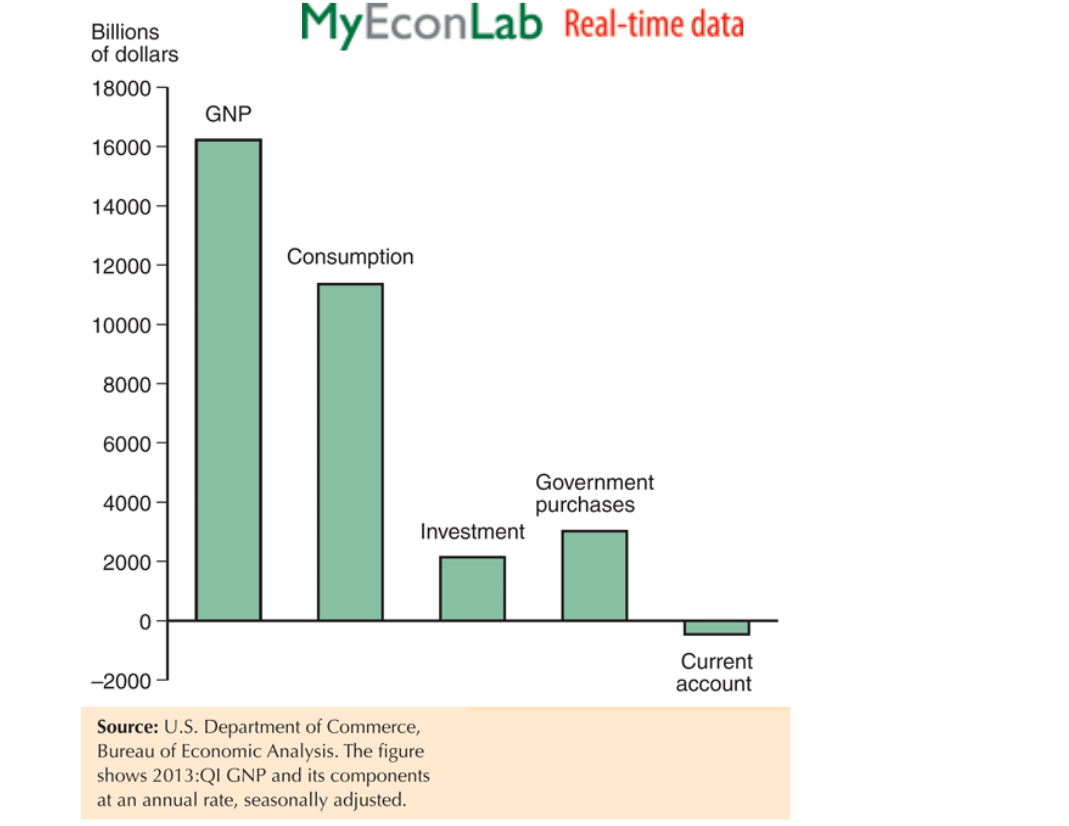
\includegraphics[scale=0.25]{gnp_us.png}
\end{figure}
}

\frame{
\frametitle{More on the Current Account}
\begin{center}
$CA = EX - IM  = Y-  \left(C + I + G \right)$
\end{center}
When production > domestic expenditure, exports > imports: current account > 0 and trade balance > 0
\begin{itemize}
\item if $Y> \left(C + I + G \right) \Rightarrow EX > IM \Rightarrow CA>0$ (surplus)
 \item if $Y< \left(C + I + G \right) \Rightarrow EX < IM \Rightarrow CA<0$ (deficit)
\end{itemize}
World production must equal world consumption, investment, and government purchases
\begin{itemize}
\item Globally, deficits and surpluses must balance
\item Some countries often borrowers, others often lenders: \textbf{global imbalances}
\end{itemize}}

\frame{
\frametitle{International Investment Position}
\begin{itemize}
    \item The stock of net foreign wealth
\end{itemize}
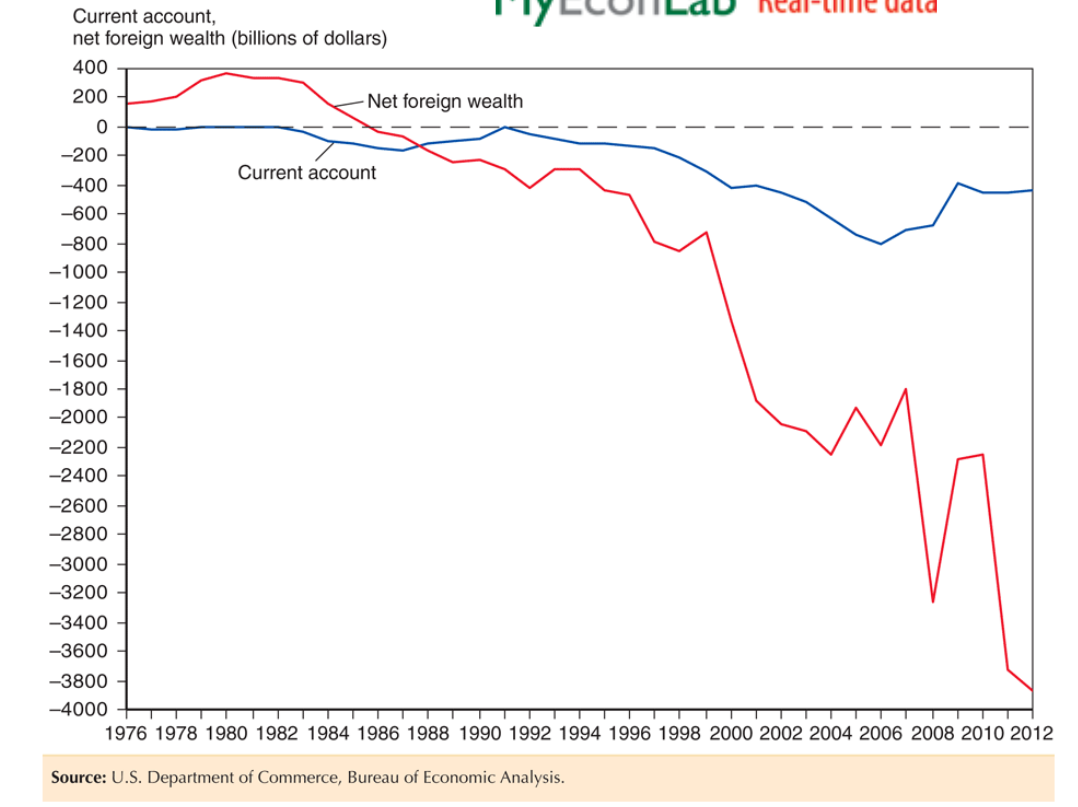
\includegraphics[scale=0.25]{iip_us.png}
\begin{itemize}
    \item Why is net foreign wealth so volatile?
\end{itemize}
}

\frame[plain]{
\frametitle{Figure; Deficits and Surpluses: The Balance of Payments (Source: IMF, International Financial Statistics)}
\begin{figure}
	\centering
		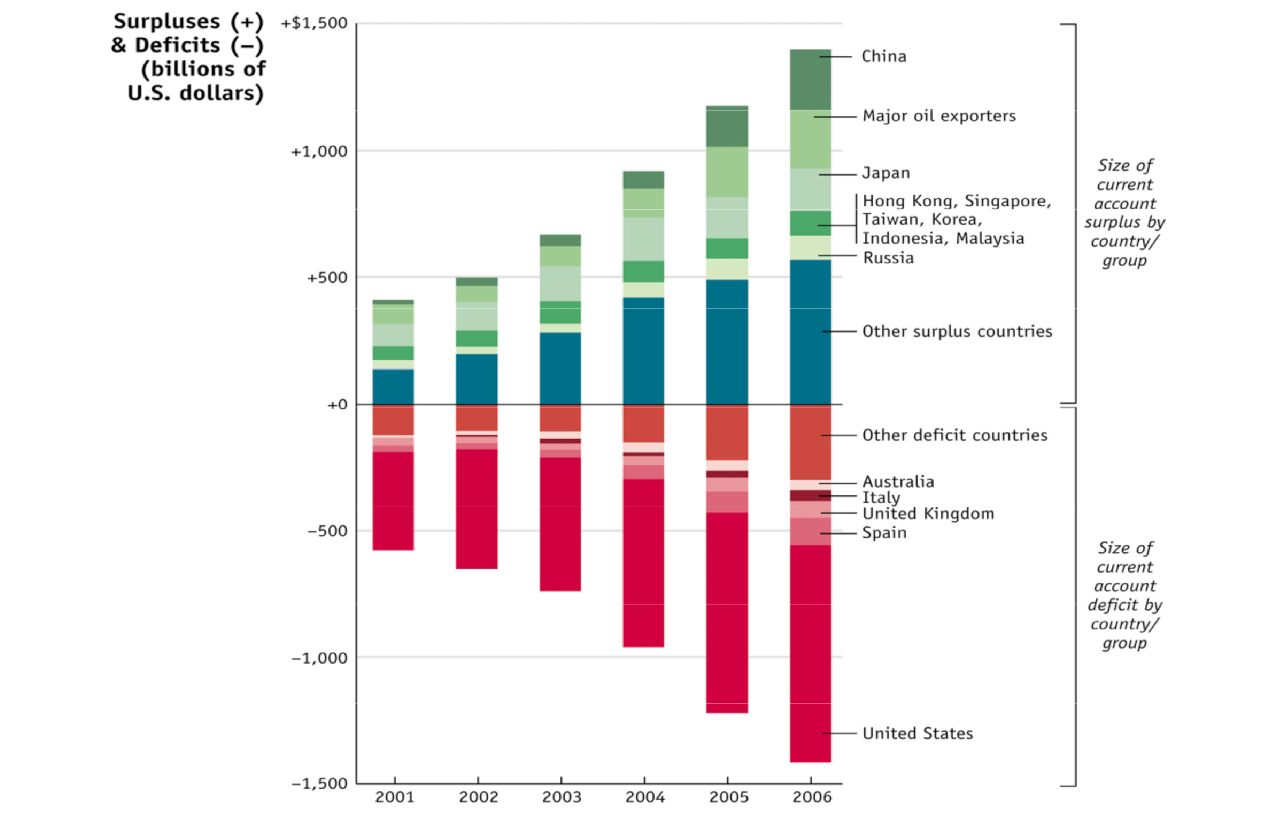
\includegraphics[scale=0.25]{imbalance_imf.png}
\end{figure}
}

\frame{
\frametitle{National Saving}
\begin{itemize}
    \item Define national savings as:
\begin{equation*}
        S=Y - C - G
\end{equation*}
    \item GNP identity:
\begin{equation*}
        Y =  C + I + G + CA
\end{equation*} 
    \item Combine the two:
\begin{equation*}
 \implies       S - CA =  I
\end{equation*}
    \item Investment can be financed by:
    \begin{enumerate}
        \item Putting off consumption (pay today)
        \item Borrowing from abroad (pay tomorrow)
        \item Current account sometimes called \emph{net foreign investment}
    \end{enumerate}
\end{itemize}
}

\frame{
\frametitle{National Saving: Private vs government}
\begin{center}
$S=Y -C -G $
\end{center}
\begin{center}
$S=\left(Y -C - T\right) + \left(T - G\right)$
\end{center}
\begin{center}
$S=S^{p} + S^{g}$
\end{center}
}

\frame{
\frametitle{National Saving: Private vs government}
\begin{itemize}
    \item Combining our two definitions of saving:
\begin{equation*}
    S = I + CA = S^{p} + S^{g}
\end{equation*}
\begin{equation*}
    S^{p} = I + CA - S^g 
\end{equation*}
\begin{equation*}
    S^{p} = I + CA + \left(G - T\right)
\end{equation*}
\item Private saving is used for: 
\begin{enumerate}
    \item Investment at home
    \item Investment abroad
    \item Purchasing government debt
\end{enumerate}
\end{itemize}
}

\begin{frame}{Pause}
    \begin{itemize}
        \item National Income Accounts
        \begin{itemize}
            \item $GNP: Y = C + I + G + CA$
            \item Only count stuff produced by factors owned by nationals
            \item Investment can be funded by foreign borrowing
        \end{itemize}
        \item Next: Balance of Payment Account
        \begin{itemize}
            \item Tracks credits and liabilities between countries 
            \item Similar to a balance sheet from accounting
        \end{itemize}
    \end{itemize}
\end{frame}

\frame{
\frametitle{Balance of Payments Accounts }
\begin{itemize}
    \item Two types of transactions:
    \begin{enumerate}
        \item Credit if a foreigner pays a native
        \item Debit if a native pays a foreigner
    \end{enumerate}
    \item A \emph{Financial Asset} holds wealth: stocks, bonds, debt, etc
    \item current account + financial account + capital account = 0
    \begin{enumerate}
\item \textbf{current account}:  tracks flows of goods and services (imports and exports)
\item \textbf{financial account}:  tracks flows of financial assets (financial capital)
\item \textbf{capital account}:  flows of special categories of assets:  typically intangible assets like debt forgiveness, copyrights and trademarks.
\end{enumerate}
\end{itemize}
}

\frame{
\frametitle{Example 1: US imports fax machine}
\begin{itemize}
    \item US imports fax machine from Italy
    \item Italian firm deposits USD in US bank
\end{itemize}
\begin{figure}
	\centering
		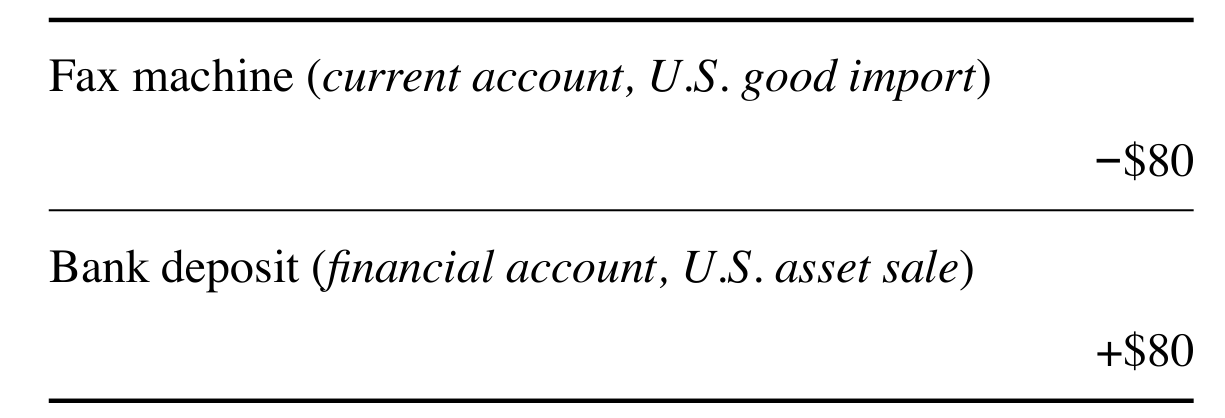
\includegraphics[width=0.85\textwidth]{num1.png}
\end{figure}
}

\frame{
\frametitle{Example 2: US tourist buys French lunch}
\begin{itemize}
    \item US tourist buys lunch in Paris
    \item Pays with US credit card
\end{itemize}
\begin{figure}
	\centering
		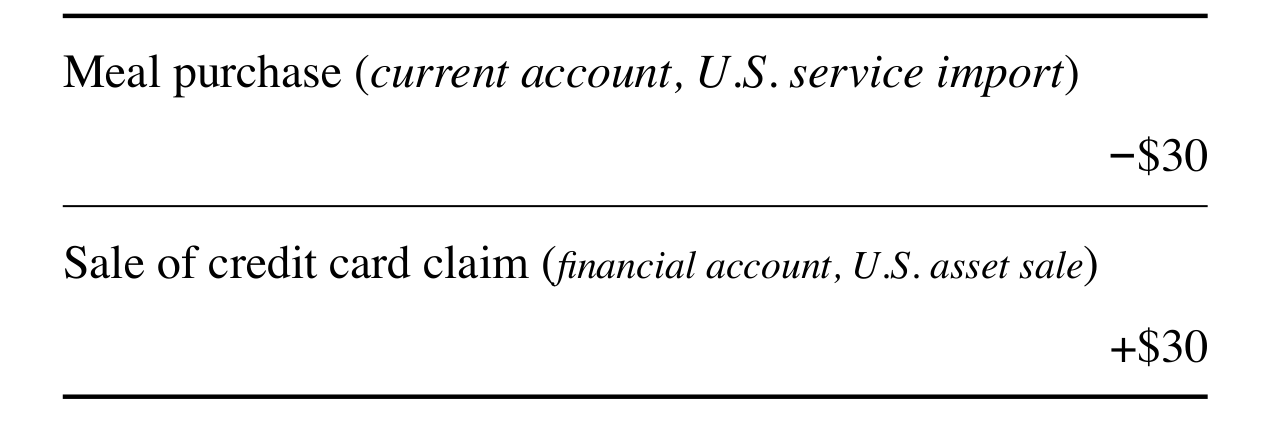
\includegraphics[width=0.85\textwidth]{num2.png}
\end{figure}
}

\frame{
\frametitle{Example 3: American buys share of British Petroleum}
\begin{itemize}
    \item American buys a share of BP
    \item BP deposits money in American bank
\end{itemize}
\begin{figure}
	\centering
		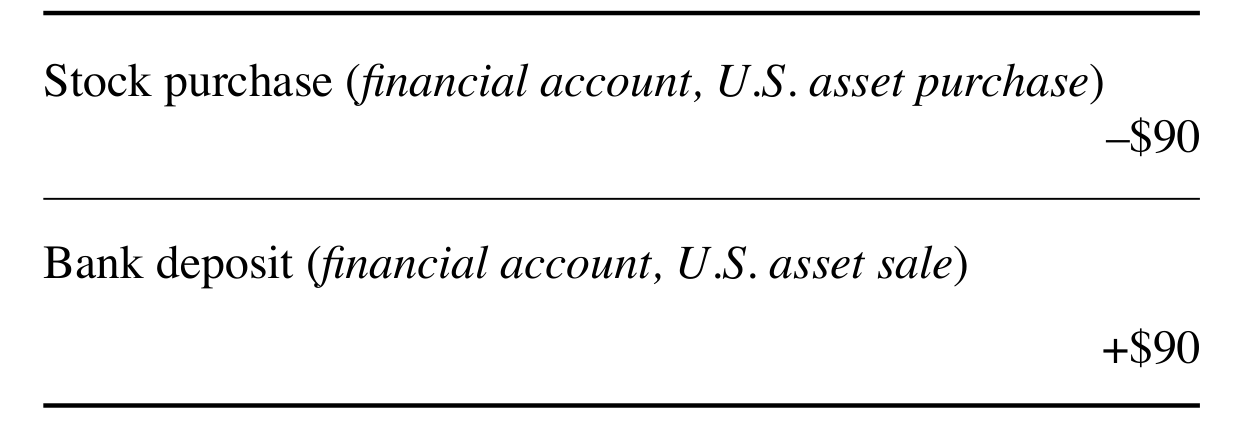
\includegraphics[width=0.85\textwidth]{num3.png}
\end{figure}
}

\frame{
\frametitle{U.S. Balance of Payments Accounts for 2012 (billions of dollars)}
\begin{figure}
	\centering
		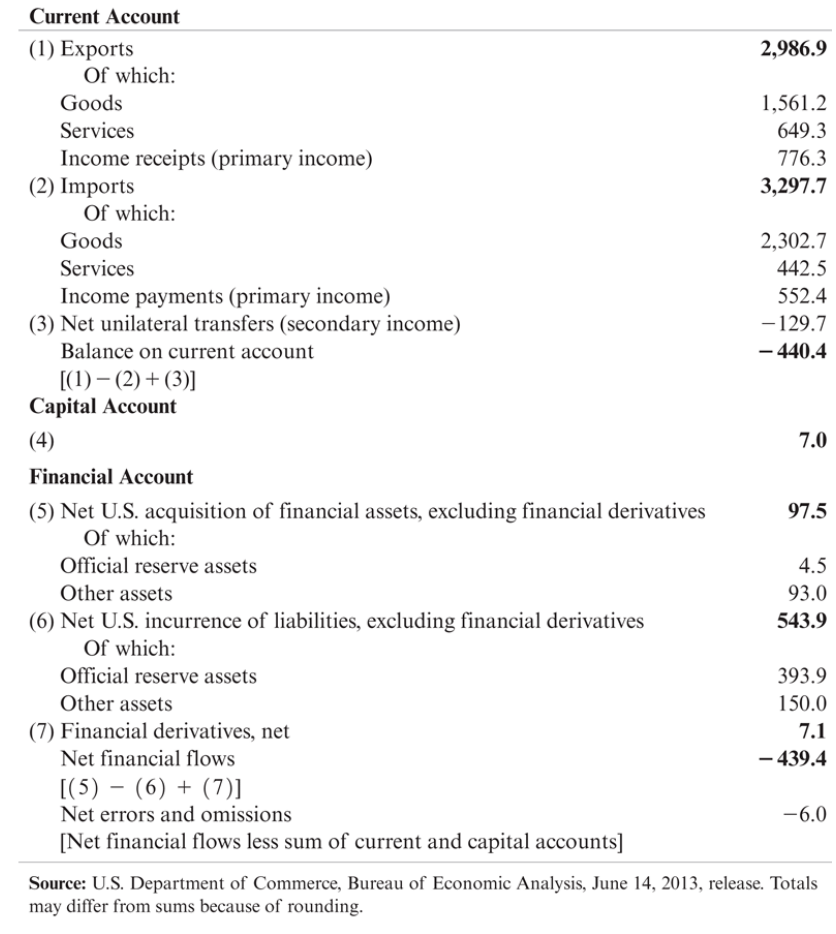
\includegraphics[scale=0.23]{bop_2012.png}
\end{figure}
}

\frame{
\frametitle{Official reserve assets}
\begin{itemize}
    \item Central banks hold foreign currency reserves
    \begin{itemize}
        \item Purpose: Insure against macroeconomic fluctuations
    \end{itemize}
    \item These are often American Treasury bills (promises that the American government will pay a dollar tomorrow)
    \item Buying and selling these bills locally allows central banks to affect money supply
\end{itemize}
}

\begin{frame}{Pause}
    \begin{itemize}
        \item National Income Accounts
        \begin{itemize}
            \item $GNP: Y = C + I + G + CA$
            \item Only count stuff produced by factors owned by nationals
            \item Investment can be funded by foreign borrowing
        \end{itemize}
        \item Next: Balance of Payment Account
        \begin{itemize}
            \item Tracks credits and liabilities between countries 
            \item Similar to a balance sheet from accounting
        \end{itemize}
    \end{itemize}
\end{frame}
% 
% \Section{Chapter 14. Exchange Rates and the Foreign Exchange Market: An Asset Approach}
% \frame[plain]{% how to print
% \frametitle{}
% \begin{center}
% \textcolor{blue}{\Huge{\textbf{Chapter 14: Exchange Rates and the Foreign Exchange Market: An Asset Approach
% }}}
% \end{center}
% }
% 
% 
% \Section{Chapter 14. Exchange Rates}
% \frame{
% \frametitle{Exchange Rates}
% If you live in Denmark:
% \begin{itemize}
% \item \textbf{Direct}: The price of the foreign currency in terms
% of DKK (e.g., $7.45$ DKK per Euro): $E_{DKK/EURO}$
% \item \textit{Indirect} : The price of DKK in terms of the foreign currency (e.g., $0.13$ Euro per 1 DKK)
% \end{itemize}
% Exchange rate regimes:
% \begin{itemize}
% \item \textit{flexible}: Exchange rate is
% determined by the market
% \item \textit{fixed}: Exchange rate is
% politically determined
% \end{itemize}
% }
% 
% \frame{
% \frametitle{Figure: Fixed and Floating Exchange Rate }
% \begin{figure}
% 	\centering
% 		\includegraphics[width=0.85\textwidth]{fixed.pdf}
% 	\label{fig:11}
% \end{figure}
% }
% 
% \frame{
% \frametitle{Table 14-1: Exchange Rate Quotations}
% \begin{figure}
% 	\centering
% 		\includegraphics[width=0.85\textwidth]{exrate.pdf}
% 	\label{fig:11}
% \end{figure}
% }
% 
% \frame{
% \frametitle{Depreciation and Appreciation}
% We are under \textbf{flexible exchange rates}:
% \begin{enumerate}
% \item \textbf{Depreciation} $E_{DKK/EURO} \Uparrow$ the Euro becomes more
% expensive, i.e., DKK becomes less valuable.
% \item \textbf{Appreciation} $E_{DKK/EURO} \Downarrow$ the Euro becomes less
% expensive, i.e., DKK becomes more
% valuable.
% \end{enumerate}
% }
% 
% 
% \frame{
% \frametitle{Devaluation and Revaluation}
% We are under \textbf{fixed exchange rates}:
% \begin{enumerate}
% \item \textbf{Devaluation} $E_{DKK/EURO} \Uparrow$ the Euro becomes more
% expensive, i.e., DKK becomes less valuable.
% \item \textbf{Revaluation} $E_{DKK/EURO} \Downarrow$ the Euro becomes less
% expensive, i.e., DKK becomes more
% valuable.
% \end{enumerate}
% }
% 
% 
% \Section{Chapter 14. The Foreign Exchange Market}
% 
% \frame{
% \frametitle{The Foreign Exchange Market}
% Four actors:
% \begin{enumerate}
% \item \textbf{Commercial banks and other depository institutions}: transactions involve buying/selling of deposits in different currencies for investment purposes.
% \item \textbf{Non-bank financial institutions} may buy/sell foreign assets for investment.
% \item \textbf{Non-financial businesses} conduct foreign currency transactions to buy/sell goods, services and assets
% \item \textbf{Central banks} conduct official international reserves transactions
% \end{enumerate}
% ICT and the integration of markets imply that there is no significant \textit{arbitrage}(=buying at a low price and selling at a high price for a profit) between markets.
% }
% 
% \frame{
% \frametitle{When Exchange Rates Misbehave (1)}
% \begin{itemize}
% \item \textbf{Exchange rate crises} occur when a currency experiences a sudden decrease in value against another currency.
% \begin{itemize}
% \item Such crises are fairly common � 19 crises 1980-2002
% \end{itemize}
% \item Crises can have severe economic consequences.
% \begin{itemize}
% \item Government default
% \item Financial and banking collapses
% \item Severe contraction in output and decline in real wages
% \end{itemize}
% \item Politically embarrassing
% \begin{itemize}
% \item Countries experiencing crises often seek help from international development agencies, such as the International Monetary Fund (IMF).
% \end{itemize}
% \end{itemize}}
% 
% \frame[plain]{
% \frametitle{When Exchange Rates Misbehave (2). Source: IMF, International Financial Statistics.
% }
% \begin{figure}
% 	\centering
% 		\includegraphics[width=0.85\textwidth]{exratemis.pdf}
% 	\label{fig:11}
% \end{figure}
% }
% 
% \frame[plain]{
% \frametitle{Case Study: Argentina (2001)
% }
% \begin{figure}
% 	\centering
% 		\includegraphics[width=0.85\textwidth]{argentina.pdf}
% 	\label{fig:11}
% \end{figure}
% }
% 
% \frame{
% \frametitle{Spot and Forward Rates}
% \begin{itemize}
% \item \textbf{Spot rates}: exchange rates for currency exchanges "on the spot", or when trading is executed in the present.
% \item \textbf{Forward rates}:  may buy/sell foreign assets for investment.
% \end{itemize}
% Other methods:
% \begin{enumerate}
% \item Foreign exchange swaps
% \item Futures contracts
% \item Options contracts
% \end{enumerate}
% }
% 
% 
% \frame{
% \frametitle{Fig. 14-1: Dollar/Pound Spot and Forward Exchange Rates, 1981-�2009 }
% \begin{figure}
% 	\centering
% 		\includegraphics[width=0.85\textwidth]{131new.pdf}
% 	\label{fig:11}
% \end{figure}
% }
% 
% \Section{Chapter 14. The Demand of Currency Deposits}
% 
% \frame{
% \frametitle{The Demand of Currency Deposits (1)}
% Factors that influence the return on assets determine the demand of those assets.
% \begin{itemize}
% \item \textbf{Rate of return:} the \% change in value that an asset offers during a time period
% \item \textbf{Real rate of return:} inflation-adjusted rate of return
% \item if inflation=0 $\Rightarrow$ rate of return=real rate of return
% \end{itemize}
% }
% 
% 
% \frame{
% \frametitle{The Demand of Currency Deposits (2)}
% Example:
% Should we invest in a Danish bond or an Euro bond?
% \begin{itemize}
% \item 1 DKK in DK bonds $\Rightarrow \left(1+R_{DKK,t}\right)$ DKK in a year
% \item 1 DKK in Euro bonds: $\Rightarrow \left(\frac{1}{E_{DKK/EURO,t}}\right)\left(1+R_{EURO,t}\right)$
% \item at time $t+1$: $\Rightarrow E^{e}_{DKK/EURO,
% t+1}\left(\frac{1}{E_{DKK/EURO,t}}\right)\left(1+R_{EURO,t}\right)$
% \item No arbitrage: the two returns have to be equal
% \end{itemize}
% }
% 
% 
% \frame{
% \frametitle{The Uncovered Interest Parity (1)}
% We can rewrite the relation as:
% \begin{center}
% $\left(1+R_{DKK,t}\right)=E^{e}_{DKK/EURO,t+1}\left(\frac{1}{E_{DKK/EURO,t}}\right)\left(1+R_{EURO,t}\right)$
% \end{center}
% \begin{center}
% $\Rightarrow$
% \end{center}
% \begin{center}
% $\left(1+R_{DKK,t}\right)=\left(1+R_{EURO,t}\right)\left(\frac{E^{e}_{DKK/EURO,t+1}}{E_{DKK/EURO,t}}\right)$
% \end{center}
% Taking logs,
% \begin{center}
% $R_{DKK,t}\approx R_{EURO,t}+\left(\frac{E^{e}_{DKK/EURO,t+1}-E_{DKK/EURO,t}}{E_{DKK/EURO,t}}\right)$
% \end{center}
% }
% 
% 
% 
% \frame{
% \frametitle{The Uncovered Interest Parity (2)}
% In other words, arbitrage ensures
% that the domestic interest rate
% equals the foreign interest rate plus
% the expected percentage
% depreciation of the domestic
% currency.
% \begin{itemize}
% \item $E^{e}_{DKK/EURO,t+1}=E_{DKK/EURO,t} \Rightarrow R_{DKK,t}=R_{EURO,t}$
% \end{itemize}
% }
% 
% 
% \frame{
% \frametitle{Table 14-3: Comparing Dollar Rates of Return on Dollar and Euro Deposits}
% \begin{figure}
% 	\centering
% 		\includegraphics[width=0.90\textwidth]{133.pdf}
% 	\label{fig:11}
% \end{figure}
% }
% 
% 
% \frame{
% \frametitle{Equilibrium in the Foreign
% Exchange Market}
% The Equilibrium Exchange Rate
% \begin{itemize}
% \item Exchange rates always adjust to
% maintain interest parity.
% \item Assume that the DKK interest rate
% $R_{DKK}$, the Euro interest rate $R_{EURO}$, and
% the expected future DKK/EURO
% exchange rate $E_{e}$, are all given
% \end{itemize}
% }
% 
% \frame{
% \frametitle{Table 14-4: }
% \begin{figure}
% 	\centering
% 		\includegraphics[width=0.90\textwidth]{135.pdf}
% 	\label{fig:11}
% \end{figure}
% }
% 
% \frame{
% \frametitle{Fig. 14-3}
% \begin{figure}
% 	\centering
% 		\includegraphics[width=0.90\textwidth]{fig133.pdf}
% 	\label{fig:11}
% \end{figure}
% }
% 
% 
% \frame{
% \frametitle{The Current Exchange Rate and the Expected Rate of Return on Dollar Deposits}
% \begin{figure}
% 	\centering
% 		\includegraphics[width=0.90\textwidth]{fig134.pdf}
% 	\label{fig:11}
% \end{figure}
% }
% 
% 
% \frame{
% \frametitle{Fig. 14-4: Determination of the Equilibrium Dollar/Euro Exchange Rate}
% \begin{figure}
% 	\centering
% 		\includegraphics[width=0.90\textwidth]{fig135.pdf}
% 	\label{fig:11}
% \end{figure}
% }
% 
% 
% \frame{
% \frametitle{Model of Foreign Exchange Markets }
% The effects of changing interest rates: 
% \begin{itemize}
% \item an increase in the interest rate paid on deposits denominated in a particular currency will increase the rate of return on those deposits. 
% \item this leads to an appreciation of the currency.
% \end{itemize}
% }
% 
% \frame{
% \frametitle{Fig. 13-5: Effect of a Rise in the Dollar Interest Rate}
% \begin{figure}
% 	\centering
% 		\includegraphics[width=0.90\textwidth]{fig136.pdf}
% 	\label{fig:11}
% \end{figure}
% }
% 
% 
% 
% 
% \frame{
% \frametitle{The Effect of an Expected Appreciation of the Euro}
% \begin{figure}
% 	\centering
% 		\includegraphics[width=0.90\textwidth]{138.pdf}
% 	\label{fig:11}
% \end{figure}
% }
% 
% \frame{
% \frametitle{Suggested Articles}
% \begin{footnotesize}
% \begin{thebibliography}{aaaaaaaaaaaaaaaaa}
% \beamertemplatearticlebibitems
% \bibitem[Jones]{jones1982}
% Barro, R.
% \newblock The Ricardian approach to budget deficits,
% \newblock The Journal of Economic Perspectives 3 (2)., 1989
% \beamertemplatearticlebibitems
% \bibitem[Jones]{jones1982}
% Burda, M.C., Severgnini, B.
% \newblock Solow Residuals without Capital Stocks,
% \newblock Journal of Development Economics, 2014
% \beamertemplatearticlebibitems
% \bibitem[Jonesa]{jonesa1982}
% Giavazzi, F., Pagano, M.
% \newblock Non-Keynesian Effects of Fiscal Policy Changes: International Evidence and the Swedish Experience
% \newblock Swedish Economic Policy Review, 3, 67-103, 1996
% \end{thebibliography}
% \end{footnotesize}
% }


\end{document}


